\documentclass{article}
\usepackage[margin=1in]{geometry}
\usepackage{amsmath}
\usepackage{booktabs}
\usepackage{float}
\usepackage{graphicx}
\usepackage{tikz}
\usetikzlibrary{arrows.meta}
\usepackage[hidelinks]{hyperref}

\title{Utility-Based Cache Partitioning}
\author{}
\date{}

\begin{document}
\maketitle


\section{Introduction}
Utility-based cache partitioning assigns shared-cache capacity according to how much each core benefits from it. A core that accesses many different blocks does not necessarily need more cache: if those blocks are not reused, extra capacity provides little benefit.

Our dynamic partitioning design is derived from Qureshi and Patt's UCP paper~\cite{ucp}. We monitor hits at different recency positions, use the estimated utility to allocate ways, and enforce the allocation during replacement. The implementation uses the active cache for monitoring and a one-way greedy allocator. It does not implement the paper's independent utility monitors or lookahead algorithm.


\begin{figure}[H]\centering
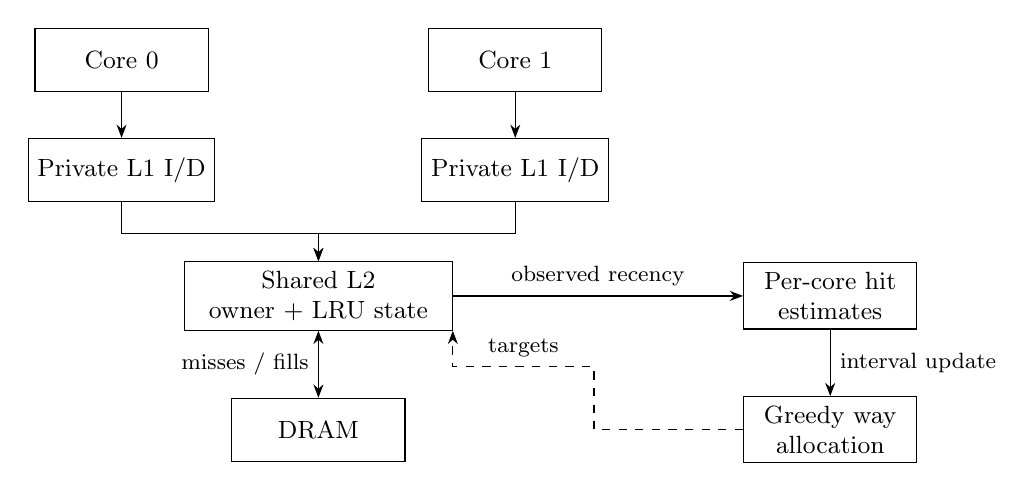
\begin{tikzpicture}[>=Stealth,font=\small,block/.style={draw,minimum width=2.2cm,minimum height=.8cm,align=center}]
\node[block] (c0) at (0,0) {Core 0};
\node[block] (c1) at (5,0) {Core 1};
\node[block] (l0) at (0,-1.4) {Private L1 I/D};
\node[block] (l1) at (5,-1.4) {Private L1 I/D};
\node[block,minimum width=3.4cm] (l2) at (2.5,-3) {Shared L2\\owner + LRU state};
\node[block] (dram) at (2.5,-4.7) {DRAM};
\node[block] (umon) at (9,-3) {Per-core hit\\estimates};
\node[block] (alloc) at (9,-4.7) {Greedy way\\allocation};
\draw[->] (c0)--(l0); \draw[->] (c1)--(l1);
\draw[->] (l0.south)--++(0,-.4)-|(l2.north);
\draw[->] (l1.south)--++(0,-.4)-|(l2.north);
\draw[<->] (l2)--node[left,font=\footnotesize]{misses / fills}(dram);
\draw[->] (l2.east)--node[above,font=\footnotesize]{observed recency}(umon.west);
\draw[->] (umon)--node[right,font=\footnotesize]{interval update}(alloc);
\draw[->,dashed] (alloc.west)--(6,-4.7)--(6,-3.9)-|node[pos=.25,above,font=\footnotesize]{targets} (l2.south east);
\end{tikzpicture}

\caption{Memory hierarchy and dynamic partitioning control. Hit estimates are collected from the active L2; allocated ways guide replacement through occupancy targets.}\label{fig:architecture}
\end{figure}

\section{Utility Monitoring}
On a cache hit, we count how many valid lines in the set have a newer LRU timestamp. This gives the hit's recency position $k$. Under the LRU stack interpretation, a cache with more than $k$ ways would retain that line.

The vector \texttt{hits\_per\_size[i]} counts hits attributed to a capacity of $i+1$ ways. For a hit at position $k$, we increment entries $k$ through $W-1$, where $W$ is the associativity. For example, in a four-way set, a hit with two more-recent lines increments entries 2 and 3. Misses increase the access count but do not increase any hit bucket.

We keep a separate vector for each core. Recency is measured in the shared set, so another core's accesses affect the estimate. This avoids separate shadow tag arrays, but the estimates depend on the current partition and interference between the cores.

\section{Dynamic Way Allocation}
Every \texttt{UMON\_INTERVAL} monitored accesses, we recompute the allocation. The current code sets this interval to 1,000,000 accesses and clears the counters after each update.

Let $U_c(q)$ be the estimated hits for core $c$ with $q$ ways, with $U_c(0)=0$. We start with zero allocated ways and assign each next way to the core with the larger gain
\[
\Delta U_c=U_c(q_c+1)-U_c(q_c).
\]
Ties go to core 0. For the example curves $[100,250,380,450]$ and $[80,200,350,480]$, the greedy choices give three ways to core 0 and one to core 1, for an estimated 460 hits.

This rule is simple, but it is not always optimal. A core may need several extra ways before it gains any hits, which a one-way comparison can miss. A shorter monitoring interval would react faster to changes but would also use fewer accesses per estimate.

\section{Partition Enforcement}
Static partitioning uses a quota within each set. Dynamic partitioning instead tracks total occupancy across the cache. The fields \texttt{ways\_allocated[c]} and \texttt{global\_occupancy[c]} hold the target way count and the current number of resident lines for each core. For $S$ sets, core 0's target is
\[
T_0=\texttt{ways\_allocated[0]}\times S.
\]
On a miss, replacement proceeds as follows:
\begin{enumerate}
\item Use an invalid entry if one is available.
\item Compare core 0's occupancy with $T_0$. If it is below target, select core 1 as the victim owner; if above target, select core 0. At the target, select the requesting core.
\item Evict the LRU line belonging to that owner in the accessed set.
\item If that owner has no line in the set, evict from the other owner.
\end{enumerate}
Global occupancy allows the ownership distribution to vary from set to set. The fallback is needed because a cache-wide target does not guarantee that the selected owner has a line in the particular set being accessed.

Monitoring, victim selection, and the two-core allocation pass each take $O(W)$ work. The utility vectors use $CW$ counters: 32 for two cores and 16 ways.

\section{Results}
The partitioning runs use two cores sharing a 512 KiB, 16-way L2. The workload pairs are bzip2+libq, bzip2+lbm, and lbm+libq, with the first workload on core 0. Table~\ref{tab:cache} adds the two reported core IPC values. Static columns give core 0's quota in ways.

\begin{table}[H]\centering\small
\begin{tabular}{lrrrrr}
\toprule
Mix & LRU & Static 4 & Static 8 & Static 12 & Dynamic \\
\midrule
mix1 & 1.276 & 1.231 & 1.288 & 1.317 & 1.166 \\
mix2 & 1.342 & 1.361 & 1.387 & 1.393 & 1.213 \\
mix3 & 1.029 & 1.028 & 1.051 & 1.083 & 1.045 \\
\bottomrule\end{tabular}\caption{Sum of the separately reported core IPCs.}\label{tab:cache}\end{table}

\begin{figure}[H]\centering
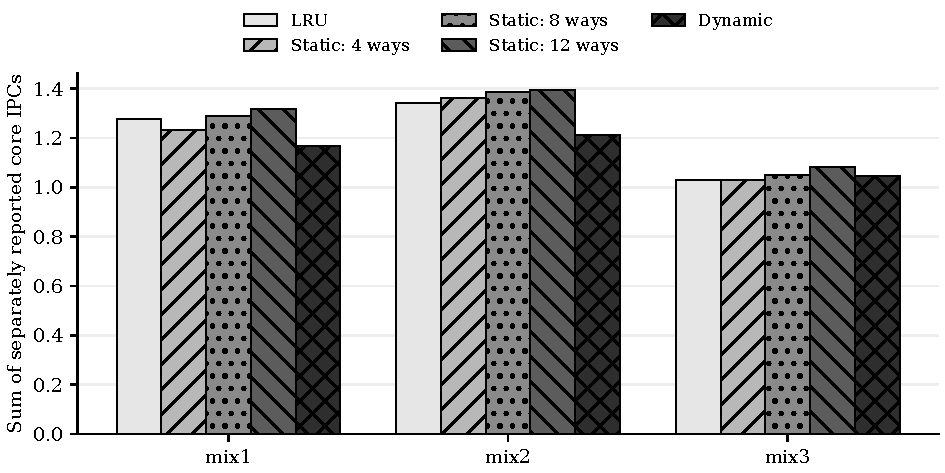
\includegraphics[width=\linewidth]{figures/partitioning_ipc.pdf}
\caption{Sum of the per-core IPC values. Static labels give the way quota for core 0; the sum is not weighted speedup.}\label{fig:results}
\end{figure}

Dynamic partitioning gives lower sums than LRU for mixes 1 and 2, by about 8.6\% and 9.6\%. It improves mix 3 by about 1.6\%. The static twelve-way allocation gives the highest sum among the configurations tested for all three mixes. The current utility estimates and greedy allocation therefore do not consistently improve these workloads. The table is a sum of per-core IPCs, not weighted speedup or IPC over a common execution interval.


\begin{thebibliography}{1}
\bibitem{ucp} Moinuddin K. Qureshi and Yale N. Patt.
\emph{Utility-Based Cache Partitioning: A Low-Overhead, High-Performance, Runtime Mechanism to Partition Shared Caches}.
MICRO, 2006.
\href{https://bpb-us-e1.wpmucdn.com/sites.gatech.edu/dist/8/175/files/2015/08/MICRO-2006-Qureshi-DynamicSetSampling.pdf?bid=175}{Paper PDF}.
\end{thebibliography}


\end{document}
